\subsection{Performance Comparison}
\label{subsec:performanceComparisonDiscussion}

%\textbf{COHEN: How did the program performance compare to its selected standard?} 
%\textbf{Did the program demonstrate good performance?}
%\textbf{Is the programs performance different from predictions?} 
%\textbf{Did you learn what you wanted from the experiments?}

The best route set, having four routes, constructed by the proposed method (SSO), is illustrated in Fig. \vref{fig:bestRouteSet4}. The best, worst, average, median produced results with the standard deviation of SSO and ACO can be found in Appendix \ref{appendixC}, Table \vref{table:performanceComparison_ACOFull}. The SSO is identical to the plain ACO implementation, but with the additional attributes inspired by PSO and BCO, in addition to the memory attribute. By using an otherwise identical algorithm enables directly comparing the performance of the two algorithms. 

First of all, it is important to acknowledge that the classic ACO has many advantages in solving VRPs. Solving certain types of NP-hard problems in polynomial time, and being optimal given there is no absolutely correct solution are some of these advantages[ref]. Before any distinct pheromone trail is laid, the ant's choices are more random and thus they perform a broad search in the environment. This randomness will decrease over time as the pheromone trails become more distinct. Because pheromone evaporate over time, shorter paths will be favored over longer paths simply because shortest paths takes shorter time. This approach is good enough when the problem to be solved is to be optimal. However, for the UTRP problem, the problem to be solved is the attempt of finding the best possible solution. In ACO the short paths will be excessively attractive to the following ones, which may result in obtaining a local optima. In the UTRP there are many factors for determining a good solution. As mentioned, a good route set is the one with the best results concerning the performance criteria. The evaluation of the route set as a whole is done after each iteration, and this evaluation will determine how good the produced route set is. Because standard ACO doesn't have a function of rewarding the best route sets, there will be no possibility to ``inform'' the ants if they are converging towards a local optimum. %To overcome these weaknesses of ACO and to boost the algorithms performance, attributes inspired by other approaches within swarm intelligence methods was added the proposed algorithm. %Thus, when one ant finds a good (i.e., short) path from the colony to a food source, other ants are more likely to follow that path, and positive feedback eventually leads to all the ants' following a single path.

As one can see in Table \vref{table:performanceComparison_ACOSSOBEST}, SSO performs better than ACO concerning the performance criteria. Observing Figure \ref{fig:acovssso}, the ACO performs worse than SSO already in the first iteration. A reason for this is that the ants in ACO does not possess the memory attribute. This feature enables ants to ``remember'' which nodes it has visited within the same route set. Adding this attribute makes the ants favor nodes not visited over nodes already visited, to make sure all nodes are visited within the same route set. Constraint \vref{itm:criteriaConnectedGraph} specifies that the route network must be connected, and without the memory function, ACO will produce more route networks not satisfying the constraint. This again makes ACO produce route sets that will be discarded, and not evaluated. %The lack of this attribute will thus prevent more (possible better) route sets being explored.  

 \begin{figure}[H]
    \begin{center}
    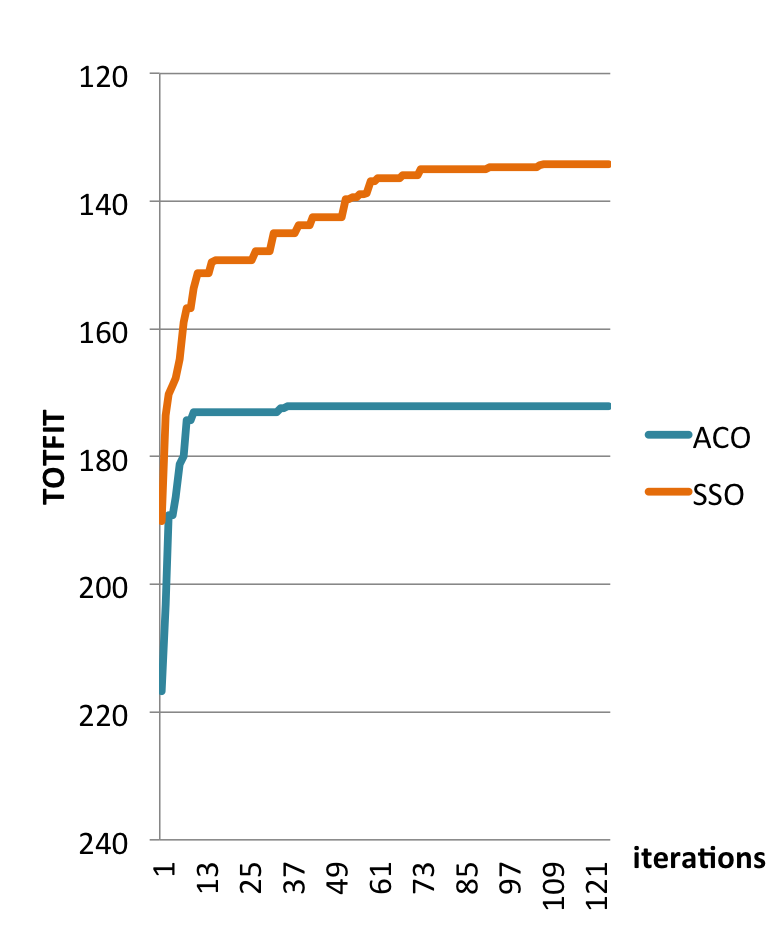
\includegraphics[width=2.5in]{assets/acovsssoNEW.png}
    \end{center}
    \caption{Evolution of TOTFIT for ACO and SSO }
    \label{fig:acovssso} 
\end{figure}

%Kan hente noe info fra setningen over?
Another reason for the performance difference is that ACO also has, as mentioned, a known shortcoming of entrapment in local optima. This disadvantage is demonstrated in Figure \ref{fig:acovssso}, which shows the average growth in the $TOTFIT$ value for each iteration. (In this figure, both algorithms are run 10 times. For each iteration the average $TOTFIT$ value for each run is recorded.) As one can observe, the ACO implementation manage to find good solutions fast, by following pheromone trails laid by previous ants. However, after approximately 35 iterations the algorithm converge towards a local optimal solution. The amount of pheromone on the initial first best routes continue to increase, and with this, unable the next ants to explore possible better solutions. 

As one can see, the proposed SSO algorithm manage to get out of this inconvenience, continuing to explore better solutions in the late iterations. As observed in the parameter settings experiment, extracted in Table \vref{table:pm2_inEvaluation}, the additional $CA$ and $AF$ parameters both improved the $TOTFIT$ value. %The parameter settings experiments were conducted to find the optimal value for these parameters. %It is worth mentioning, the experiments performed in this table was done in order to find the best parameter value for the algorithm performance, and the default value while testing for both parameters was 10\%.

\citet{kechagiopoulos14} used a particle swarm optimization (PSO) algorithm which proved to perform better than all solutions compared to. In PSO, like ACO, the particles tend to explore more in the the early iterations of the algorithm, and becoming more organized and coordinated at the late iterations. In PSO, this is due to a parameter called Inertia Weight. The parameter is added to balance the local and global search, preventing the particles from drastically changing directions. However, the best global known solution the particles are drawn against may, similar to ACO, be a (possible) local optimum. 

The attribute ``crazy ants'' is added to the proposed method, where an amount of the colony is given the possibility to explore edges completely random, and will not be influenced by the best known solutions.T he attribute $CA$ enables the algorithm to explore new (possible better) routes, regardless of the pheromone value laid on the edges. The value of $CA$ denotes the amount of ``crazy ants'' which explores edges randomly. This parameter can thus enable the algorithm to break out of a (possible) local optima. 

This additional feature improved the performance of the proposed algorithm. This may be due to the fact that the attribute enables an amount of ants to explore undetected better solutions when pheromone trails becomes too great. The Inertia Weight parameter, inspired from PSO, denotes the amount of crazy ants in the beginning of each run, and the amount of ``crazy ants'' decrease in line with the parameter. Decreasing the inertia weight in PSO may suffer from low global search ability at the end of the run, and thus the possibly of getting stuck at a local optima. However, in the proposed method the ``crazy ants'' are not searching towards the best known solution, and will thus prevent the same disadvantage. 

The reader recalls that the $AF$ parameter selects and amount of the best produced route sets of an iteration, and the following ants will basically reward these edges with more pheromone. Giving a small amount of route sets additional pheromone by the $p_b$ parameter improved the algorithms performance further. Rewarding edges in a large amount best route sets will result in over appreciating too many edges, which again will unable to distinct edges in good route sets from edges in the best route sets. 

\citet{salehi-nezhad07}, \citet{tripathi09}, and \citet{sedighpour14} all showed that rewarding the best solutions found so far improved the algorithm. Rewarding the best solution may be seen as the similar recruit function of the bee colony optimization (BCO). In BSO the artificial bee which has produced a good route set it can ``recruit'' other nest-mates, and thus inform the others that a good route set is found. This process inspired to add the ``following'' feature to the proposed method. After the route sets are evaluated, an amount of the best ants with the best route sets is selected to be followed in the next iteration. The same amount of ants will follow the same routes as the one they are following, and thus create the exact same route set. This will give the edges in the best route sets more pheromone, and thus distinct edges with much pheromone (because they are walked by many ants, given the short path) from edges that are better concerning the performance criteria. The proposed algorithm's performance was improved with this additional attribute. However, the algorithm performed best with a relatively small amount of followers, but with a large amount of pheromone.  Rewarding edges in a large amount best route sets will result in over appreciating too many edges, which again will unable to distinct edges in good route sets from edges in the best route sets.  %By making ants follow new best routes after each iteration will also give a variation of the best produced route sets, and thus avoid over rewarding edges in a local optima. 

\begin{table}
    \centering
    %\hspace*{-0.5cm}
    \begin{tabular}{|l|l|l|l||c|}
    \hline
    Parameter & $CA$ & $AF$ & $p_b$ & $AVG(TOTFIT)$ \\
    \hline
    $CA$ & \textbf{0\%} & 10\% & 0.0 & 105.66\\
    ~ & \textbf{25\%} & 10\% & 0.0 & \textbf{103.597}\\
    \hline
    $AF$ & 10\% & \textbf{0\%} & 0.0 & 105.747 \\
    ~ & 10\% & \textbf{5\%} & 0.0 & \textbf{104.389}\\
    \hline
    $p_b$ & 10\% & 5\% & \textbf{0.0} & 104.882\\
    ~ & 10\% & 5\% & \textbf{0.9} & \textbf{102.579}\\
    \hline
    \end{tabular}
    \caption {Caption}
    \tiny
    \begin{itemize}[noitemsep]
    \item[ ] $AVG(TOTFIT)$ : Average produced Total Fitness function
    %\item[$^1$:] On average \% of the iterations of each run did not create any ants that satisfied the initial Constraint \ref{itm:criteriaConnectedGraph} described in Section \vref{sec:algoConstraints}.
    \end{itemize}
    \label{table:pm2_inEvaluation}
\end{table}

%TODO:
%The ants in SSO also possess the knowledge of the global best known solution. This feature will increase the probability of the next ants selecting the edges walked by the best ant so far. Further, if a better global best known solution is found, new edges will have increased probability of being selected, and the next ants will walk towards a better global solution. As one can see in \vref{table:performanceComparison_ACOSSOGlobal_sol}, this did not improve the SSO algorithm further. 

In Table \vref{table:performanceComparison_4}, the results of the SSO, having four routes, are compared with route sets published in the literature. As one can observe in Table \vref{table:performanceComparison_4},  $d_{unsat}$ is 0, similar to all other approaches. The theoretical best value of for this criteria is 0, which reflects no passenger have to transfer more than 2 times. All approaches, except \citep{mandl79, kidwai98, chakroborty02}, performs better concerning the $d_0$, $d_1$ and $d_2$ criteria. However, the route set constructed by SSO has a better $ATT$ compared to all route sets constructed by the other approaches. The best route set, having six routes, constructed by the proposed algorithm is presented in Fig. \vref{fig:bestRouteSet6}. The best route set, having seven routes, constructed by the proposed algorithm is presented in Fig. \vref{fig:bestRouteSet7}. The best route set, having eight routes, constructed by the proposed algorithm is presented in Fig. \vref{fig:bestRouteSet8}. The performance comparison for each route set size is found in Table \vref{table:performanceComparison_6}, Table \vref{table:performanceComparison_7}, and Table \vref{table:performanceComparison_8}, respectively. As one can observe, in all route set sizes the proposed algorithm is continuing to produce a higher $ATT$ than all other approaches, and performance criteria $d_0, d_1,$ and $d_{2}$ are all below average, whereas $d_{unsat}$ is still 0. As one can observe in Table \vref{table:performanceComparison_routesets}, the amount of direct travelers increase, and the average travel time decrease in line with the number of routes. This corresponds to the growth in performance in all other approaches. The probability of finding direct routes and routes with small travel times is higher when there are more routes to select from. 

 \begin{table}[H]
    \centering
    \begin{tabular}{|l||l|l|l|l|l|}
    \hline
    Route Set & $d_0(\%)$ & $d_1(\%)$ & $d_2(\%)$ & $d_{unsat}(\%)$ & $ATT$ \\
    \hline
    4 & 85.21 & 13.49 & 1.30 & 0.00 & 10.27\\
    6 & 87.17 & 12.0 & 0.82 & 0.01 & 10.11\\
    7 & 88.49 & 10.72 & 0.79 & 0.0 & 10.08\\
    8 & 89.16 & 10.05 & 0.80 & 0.0 & 10.06\\
    \hline
    \end{tabular}
    \caption {Evaluating increase of Route Sets}
    % 50 runs
    \label{table:performanceComparison_routesets}
\end{table}

The proposed method produce the best average travel time compared to all route sets sizes published in the literature. Concerning the unsatisfied passengers criteria, there are no passengers needing to transfer more than twice in the best produced route set, which is equal to all approaches published in the literature. For the rest of the performance criteria concerning the number of direct travelers, one transfers, and two transfers, the algorithm performs below average compared to the other approaches. It is worth mentioning that neither of the algorithms we are comparing against (sjekke dette) tested their algorithms on other, larger networks. The robustness of their algorithms regarding both time and space complexity could have been verified by also applying their algorithm to a larger test case. %This is due to a user-defined parameter sat to favor a small travel time over a high amount of direct transfers, based on the ration between the two. Again, it is worth mentioning that a direct route is still an important factor when evaluating the best route set. This reflects that the number of direct travelers in the best produced route set is still relatively high.
The calculation of the evaluation function $TOTFIT$ is, as mentioned, the sum of $F1$, $F2$ and $F3$. As described in \vref{sec:f1}, a weight parameter, $\sigma$, is used to control the importance of $F1$, $F2$, and $F3$. In the proposed algorithm, $\sigma$ is sat to favor $F1$, which is directly linked to a low $ATT$. Demonstrated in Fig. \vref{fig:mandlWithTT}, when traveling from Node 7 to Node 14 the algorithm will choose to transfer from Route 4 to Route 3, which has a travel time of 20 minutes including a transfer penalty of 5 minutes. The $F2$ parameter is concerned whether the algorithm has a high $d_0$, denoting a minimum number of transfers. If $F2$ is favored over $F1$, the route set would get a lower score and not be selected as the best route set. This is because Route 1, which have a direct route from Node 7 to Node 14 with a travel time of 27 minutes. It is worth mentioning that the algorithm does not select $F1$ unconditionally, a high amount of $d_0$ is still important, but the algorithm select the best route set concerning the ratio between the two.

\begin{figure}[H]
    \begin{center}
    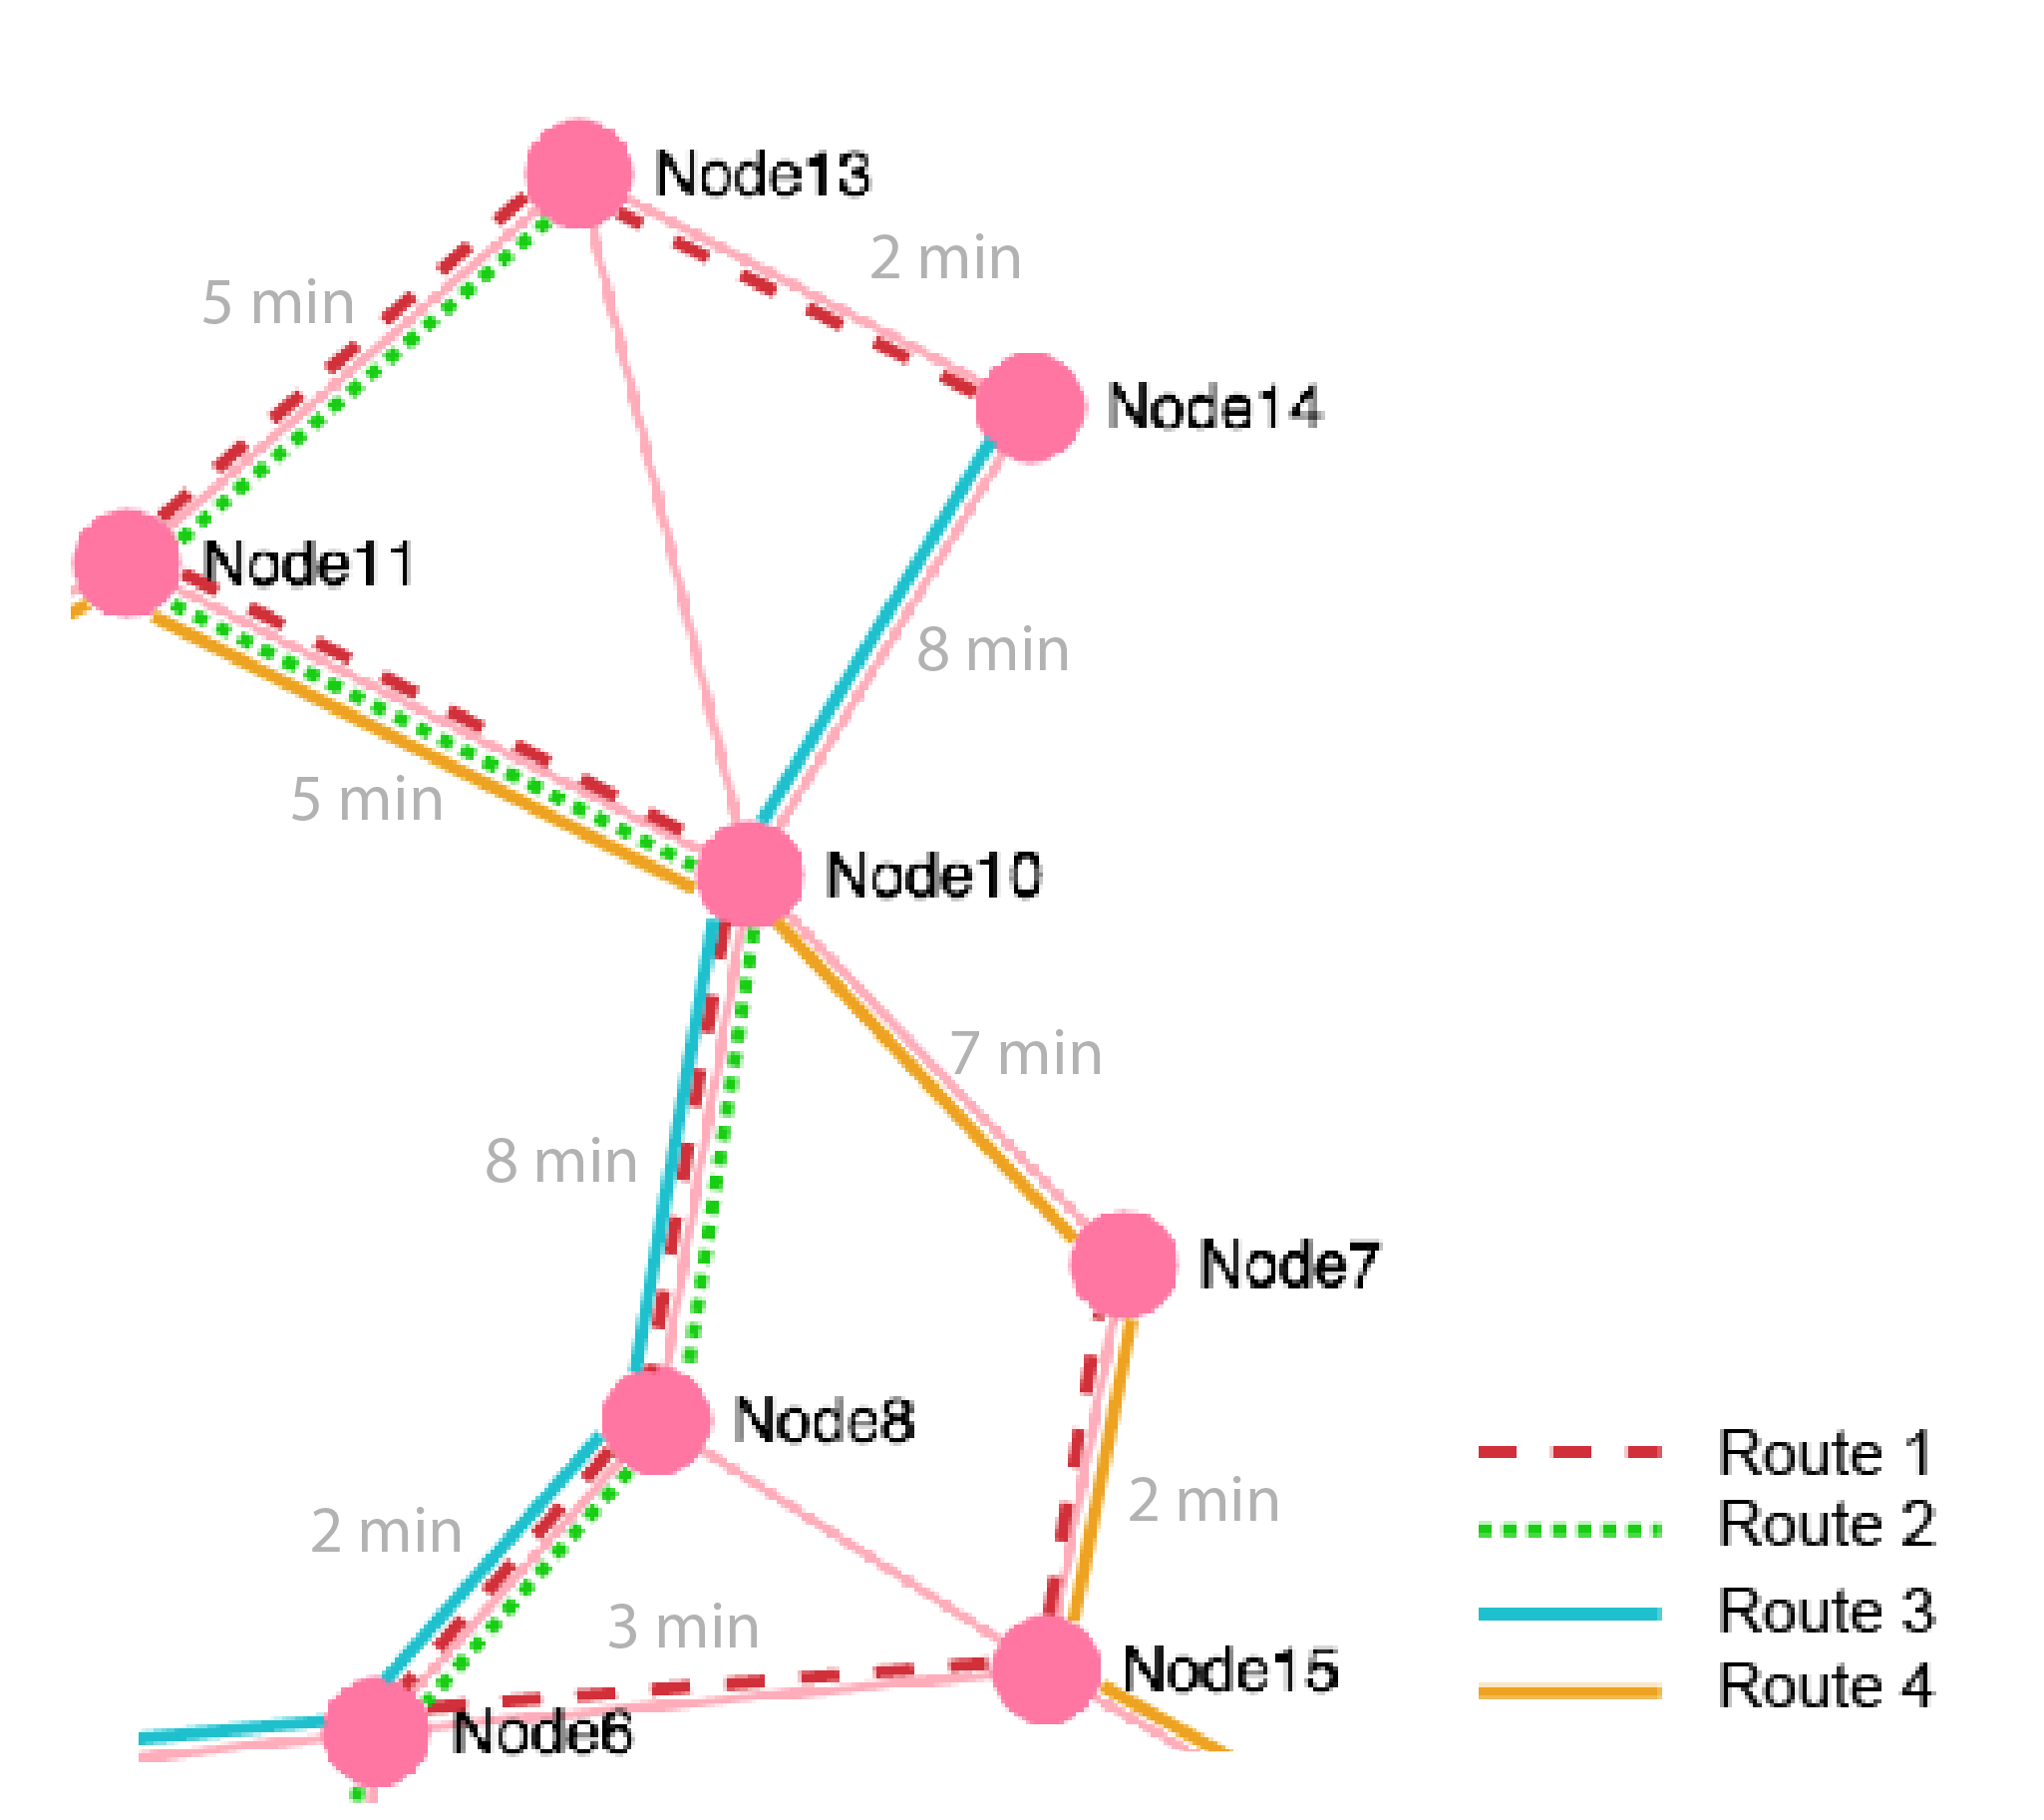
\includegraphics[width=3.5in]{assets/mandl_withTT_utsnitt.png}
    \end{center}
    \caption{A fragment of the best route set, having four route sets, constructed by the proposed algorithm including transfer times in minutes between each node.}
    \label{fig:mandlWithTT} 
\end{figure}

As mentioned in the motivation, citizens often prefer private transportation because of the decreased travel time when no detours is needed. Then again, another important issue concerning passenger satisfiability, is the issue of not needing to change vehicles during a trip. Whether a passenger would travel travel direct with a larger travel time versus transferring and thus decrease the travel time, is a matter of preferences. As you can see in all the approaches published in the literature including the proposed algorithm, you will have to choose one at the expense of the other. One can argue back and forth on the importance of each criteria. We believe that in the modern urban city, a minimum travel time is an important factor. People should have a small travel time as an option if time is limited. As mentioned, the produced route network also possess a relatively high amount of direct routes, giving passengers opportunities to choose direct routes if this is desired. %And reflecting the average travel time of the best route set produced by the proposed algorithm, the direct travels are not very long. %jeg er litt usikker på om jeg er på villspor her
When all comes to all, it is eventually up to each individual passenger choosing what is most convenient for them. 






